% Options for packages loaded elsewhere
\PassOptionsToPackage{unicode}{hyperref}
\PassOptionsToPackage{hyphens}{url}
%
\documentclass[
]{article}
\usepackage{amsmath,amssymb}
\usepackage{lmodern}
\usepackage{iftex}
\ifPDFTeX
  \usepackage[T1]{fontenc}
  \usepackage[utf8]{inputenc}
  \usepackage{textcomp} % provide euro and other symbols
\else % if luatex or xetex
  \usepackage{unicode-math}
  \defaultfontfeatures{Scale=MatchLowercase}
  \defaultfontfeatures[\rmfamily]{Ligatures=TeX,Scale=1}
\fi
% Use upquote if available, for straight quotes in verbatim environments
\IfFileExists{upquote.sty}{\usepackage{upquote}}{}
\IfFileExists{microtype.sty}{% use microtype if available
  \usepackage[]{microtype}
  \UseMicrotypeSet[protrusion]{basicmath} % disable protrusion for tt fonts
}{}
\makeatletter
\@ifundefined{KOMAClassName}{% if non-KOMA class
  \IfFileExists{parskip.sty}{%
    \usepackage{parskip}
  }{% else
    \setlength{\parindent}{0pt}
    \setlength{\parskip}{6pt plus 2pt minus 1pt}}
}{% if KOMA class
  \KOMAoptions{parskip=half}}
\makeatother
\usepackage{xcolor}
\IfFileExists{xurl.sty}{\usepackage{xurl}}{} % add URL line breaks if available
\IfFileExists{bookmark.sty}{\usepackage{bookmark}}{\usepackage{hyperref}}
\hypersetup{
  hidelinks,
  pdfcreator={LaTeX via pandoc}}
\urlstyle{same} % disable monospaced font for URLs
\usepackage[margin=1in]{geometry}
\usepackage{longtable,booktabs,array}
\usepackage{calc} % for calculating minipage widths
% Correct order of tables after \paragraph or \subparagraph
\usepackage{etoolbox}
\makeatletter
\patchcmd\longtable{\par}{\if@noskipsec\mbox{}\fi\par}{}{}
\makeatother
% Allow footnotes in longtable head/foot
\IfFileExists{footnotehyper.sty}{\usepackage{footnotehyper}}{\usepackage{footnote}}
\makesavenoteenv{longtable}
\usepackage{graphicx}
\makeatletter
\def\maxwidth{\ifdim\Gin@nat@width>\linewidth\linewidth\else\Gin@nat@width\fi}
\def\maxheight{\ifdim\Gin@nat@height>\textheight\textheight\else\Gin@nat@height\fi}
\makeatother
% Scale images if necessary, so that they will not overflow the page
% margins by default, and it is still possible to overwrite the defaults
% using explicit options in \includegraphics[width, height, ...]{}
\setkeys{Gin}{width=\maxwidth,height=\maxheight,keepaspectratio}
% Set default figure placement to htbp
\makeatletter
\def\fps@figure{htbp}
\makeatother
\setlength{\emergencystretch}{3em} % prevent overfull lines
\providecommand{\tightlist}{%
  \setlength{\itemsep}{0pt}\setlength{\parskip}{0pt}}
\setcounter{secnumdepth}{5}
\usepackage{booktabs}
\usepackage{booktabs}
\usepackage{longtable}
\usepackage{array}
\usepackage{multirow}
\usepackage{wrapfig}
\usepackage{float}
\usepackage{colortbl}
\usepackage{pdflscape}
\usepackage{tabu}
\usepackage{threeparttable}
\usepackage{threeparttablex}
\usepackage[normalem]{ulem}
\usepackage{makecell}
\usepackage{xcolor}
\ifLuaTeX
  \usepackage{selnolig}  % disable illegal ligatures
\fi

\author{}
\date{\vspace{-2.5em}}

\begin{document}

\hypertarget{simulation-controlling-underlying-data-generation-process}{%
\subsection{Simulation Controlling Underlying Data Generation Process}\label{simulation-controlling-underlying-data-generation-process}}

The fully simulated data simulation allows for insight into the behavior of the MLLT under correct and incorrect model specification. This simulation study also highlights shortcomings of independently fit LLT models when correlation exists in the observation or state equations. The data is simulated under three scenarios: 1.) correlation only exists in the observation equation (O), 2.) correlation only exists in the state equation (S), and 3.) correlation exists in both the observation and state equation (OS). The independent LLT, the O MLLT, S MLLT, and OS MLLT are all fit to each of the three data generation processes.

The covariates are randomly generated to mirror the predictors of interest (section\_\_\_\_\_\_\_). There is a time effect, a binary group effect, and a linear continuity point effect. For each simulation, 100 subjects are generated with between 2-12 observations. The ``true'' linear effects \(\boldsymbol{\beta}\), observation error covariance (\(\Sigma_\varepsilon\)), and underlying state process covariance (\(\Sigma_\eta\)) are denoted in equation (\_\_\_\_\_\_\_\_\_\_\_).

The underlying data generation for each of the three simulation scenarios are as follows,

\begin{equation*}
\begin{aligned}
\begin{bmatrix}
y_{ij1}\\
y_{ij2}\\
y_{ij3}
\end{bmatrix}
&= \begin{bmatrix}
\alpha_{ij1}\\
\alpha_{ij2}\\
\alpha_{ij3}
\end{bmatrix}
+ 
\begin{bmatrix}
\boldsymbol{x_{ij}\beta_1}\\
\boldsymbol{x_{ij}\beta_2}\\
\boldsymbol{x_{ij}\beta_3} 
\end{bmatrix} +
\begin{bmatrix}
\varepsilon_{ij1}\\
\varepsilon_{ij2}\\
\varepsilon_{ij3}
\end{bmatrix}, \ \ \ 
\begin{bmatrix}
\varepsilon_{ij1}\\
\varepsilon_{ij2}\\
\varepsilon_{ij3}
\end{bmatrix} 
\sim N(0, \Sigma_\varepsilon
)\\
\begin{bmatrix}
\alpha_{ij1}\\
\alpha_{ij2}\\
\alpha_{ij3}
\end{bmatrix} & = 
\begin{bmatrix}
\alpha_{i(j-1)1}\\
\alpha_{i(j-1)2}\\
\alpha_{i(j-1)3}
\end{bmatrix} +
\begin{bmatrix}
\eta_{ij1}\\
\eta_{ij2}\\
\eta_{ij3}
\end{bmatrix}, \ \ \
\begin{bmatrix}
\eta_{ij1}\\
\eta_{ij2}\\
\eta_{ij3}
\end{bmatrix} \sim N(0, \delta_{ij} \Sigma_\eta 
)\\
\boldsymbol{\beta} &= \begin{bmatrix} \boldsymbol{\beta_1} & \boldsymbol{\beta_2} &  \boldsymbol{\beta_3} \end{bmatrix} = 
\begin{bmatrix}
4 & -3 & 0\\
2 & 0 & 0\\
1 & 1 & 0
\end{bmatrix}
\end{aligned}
\end{equation*}

for \(i \in \{1, 2, ..., 100\}\) and \(j \in \{2, 3,..., 12\}\). The parameters in \(\boldsymbol{\beta}\) were chosen to have no, small, medium, large, and negative effects. For the three different data generation scenarios we utilize differing values of \(\Sigma_\varepsilon\) and \(\Sigma_\eta\).

\hypertarget{o-model}{%
\paragraph{O Model}\label{o-model}}

\begin{equation*}
\Sigma_\varepsilon = 
\begin{bmatrix}
15 & 2.4 & 1\\
2.4 & 15 & 1\\
1 & 1 & 10
\end{bmatrix}, \ \ \ 
\Sigma_\eta =
\begin{bmatrix}
5 & 0 & 0\\
0 & 5 & 0\\
0 & 0 & 2
\end{bmatrix}
\end{equation*}

\hypertarget{s-model}{%
\paragraph{S Model}\label{s-model}}

\begin{equation*}
\Sigma_\varepsilon = 
\begin{bmatrix}
15 & 0 & 0\\
0 & 15 & 0\\
0 & 0 & 10
\end{bmatrix}, \ \ \ 
\Sigma_\eta =
\begin{bmatrix}
5 & 3.7 & 0\\
3.7 & 5 & 0\\
0 & 0 & 2
\end{bmatrix}
\end{equation*}

\hypertarget{os-model}{%
\paragraph{OS Model}\label{os-model}}

\begin{equation*}
\Sigma_\varepsilon = 
\begin{bmatrix}
15 & 2.4 & 1\\
2.4 & 15 & 1\\
1 & 1 & 10
\end{bmatrix}, \ \ \ 
\Sigma_\eta =
\begin{bmatrix}
5 & 3.7 & 0\\
3.7 & 5 & 0\\
0 & 0 & 2
\end{bmatrix}
\end{equation*}

The covariance matrices \(\boldsymbol{\Sigma_\varepsilon}\) and \(\boldsymbol{\Sigma_\eta}\) were chosen to approximate values observed when the MLLT models were fit to real data.

For each scenario, the simulations are carried out 1000 times. The most effective model is one that is unbiased, maintains 95\% coverage, and small parameter variance (indicated by small confidence interval length) for the parameters in \(\boldsymbol{\beta}\), \(\boldsymbol{\Sigma_\varepsilon}\), and \(\boldsymbol{\Sigma_\eta}\). Maintaining proper 95\% coverage indicates proper type I error at the level of 0.05. If we can fix type I error, the next step is to minimize type II error which then leads to greater power to detect significant differences. Minimizing type II error will occurs by minimizing the parameter variance if the estimates are unbiased and have proper 95\% coverage. As we are using a Bayesian Gibb's sampling approach, the confidence interval is used to judge parameter variance.

The Bayesian Gibb's sampler is repeated 5000 times with a burn-in of 2000 for each model. This means samples 2001-5000 are used for parameter inference.

\hypertarget{fully-simulated-results}{%
\subsubsection{Fully Simulated Results}\label{fully-simulated-results}}

The LLT, O, S, and OS models all show unbiasedness and near 95\% coverage in the linear effect parameters. This occurs despite the LLT, O, and S models having a level of misspecification in the covariance parameters. In the linear effects there is not a large difference in confidence interval length between the different methods. The O, S, and OS models measure up well to the LLT.

The parameters in \(\Sigma_\varepsilon\) vary much more. The LLT and the S models assume there is not any covariance in the observation error, therefore, do not seek to estimate the non-diagonal values of \(\Sigma_\varepsilon\). Even so, the LLT and S models are fairly accurate in estimating the observation variances. The O model, which does assume observation error covariance, greatly over estimates the covariance parameters. This is because the O model assumes no covariance in the state equation, therefore, any correlation in the state equation ends up being allocated to the observation error. Additionally, we see the same principle for the S model in estimating \(\Sigma_\eta\). The covariance parameters of \(\Sigma_\eta\) are inflated as model S is assuming correlation truly occurring in \(\Sigma_\varepsilon\) is actually occurring in the underlying cognitive process.

The OS model, which is correctly specified, unsurprisingly accurately estimates the \(\Sigma_\varepsilon\) and \(\Sigma_\eta\). Similar studies were conducted, except O or S were correctly specified. When either O or S were correctly specified they slightly outperformed the OS model. This is because the OS model estimates \(K(K-1)/2\) more parameters than the other models. But, as can be seen from this simulation analysis, if O or S are misspecified it can lead to miscalculation in the covariance matrices. The OS model is much more robust in terms of handling different observation error and cognitive process correlation.

Shortcomings are also blatantly evident as the LLT provides no observation error or cognitive process correlation estimation. The O and S models do provide some insight into the inter-relatedness between cognition tests, but the OS provides the most descriptive form of the correlations. Even with the added benefits of the MLLT, it perform just as well as the LLT in modeling linear effects.

\hypertarget{o-model-1}{%
\paragraph{O Model}\label{o-model-1}}

\begin{longtable}[t]{l|l|r|r|r|r|r}
\caption{\label{tab:unnamed-chunk-8}Linear Effect Coverage}\\
\hline
Test & Variable & Beta & LLT & O & S & OS\\
\hline
Y1 & X1 & 4 & 0.964 & 0.965 & 0.969 & 0.963\\
\hline
Y1 & X2 & 2 & 0.965 & 0.964 & 0.958 & 0.957\\
\hline
Y1 & X3 & 1 & 0.953 & 0.953 & 0.955 & 0.954\\
\hline
Y2 & X1 & -3 & 0.940 & 0.948 & 0.945 & 0.943\\
\hline
Y2 & X2 & 0 & 0.955 & 0.954 & 0.952 & 0.962\\
\hline
Y2 & X3 & 1 & 0.937 & 0.932 & 0.942 & 0.938\\
\hline
Y3 & X1 & 0 & 0.957 & 0.950 & 0.954 & 0.952\\
\hline
Y3 & X2 & 0 & 0.948 & 0.949 & 0.950 & 0.956\\
\hline
Y3 & X3 & 0 & 0.950 & 0.950 & 0.949 & 0.947\\
\hline
\end{longtable}

\begin{figure}
\centering
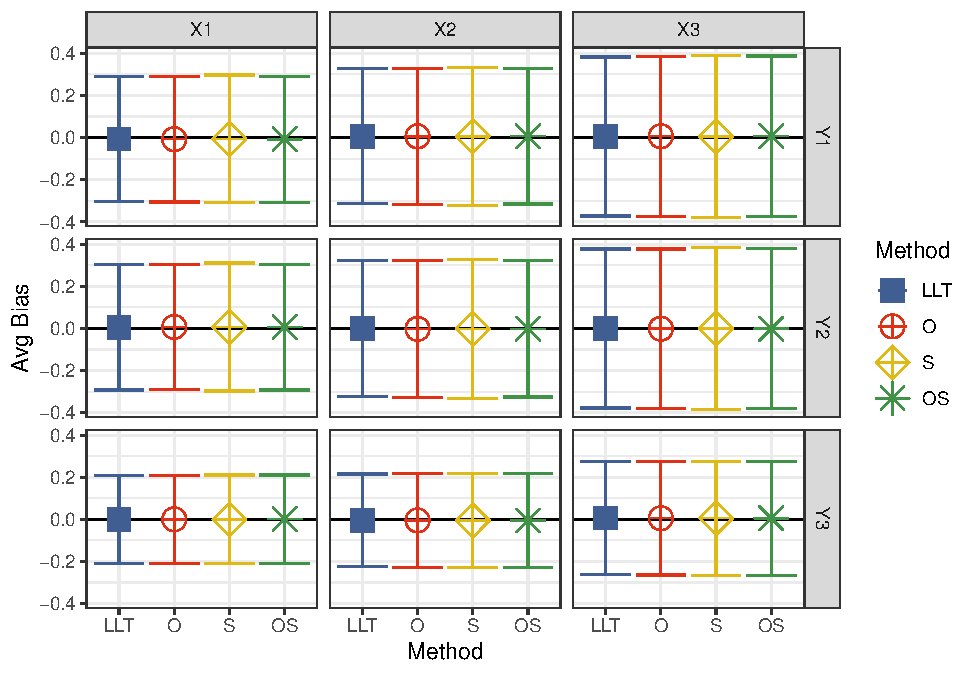
\includegraphics{FullSimulation_files/figure-latex/unnamed-chunk-9-1.pdf}
\caption{\label{fig:unnamed-chunk-9}Parameter Bias and Variablilty}
\end{figure}

\begin{longtable}[t]{l|r|l|r|l|r}
\caption{\label{tab:unnamed-chunk-10}Observation Covariance Estimates}\\
\hline
param & true & LLT & O & S & OS\\
\hline
1,1 & 15.0 & 14.909 & 14.919 & 14.688 & 14.950\\
\hline
1,2 & 2.4 & - & 2.371 & - & 2.425\\
\hline
2,2 & 15.0 & 14.892 & 14.903 & 14.668 & 14.927\\
\hline
1,3 & 1.0 & - & 0.990 & - & 1.027\\
\hline
2,3 & 1.0 & - & 0.988 & - & 1.008\\
\hline
3,3 & 10.0 & 10.056 & 10.063 & 10.021 & 10.093\\
\hline
\end{longtable}

\begin{longtable}[t]{l|l|r|l|r}
\caption{\label{tab:unnamed-chunk-11}Observation Covariance Coverage}\\
\hline
param & LLT & O & S & OS\\
\hline
1,1 & 0.95 & 0.951 & 0.928 & 0.948\\
\hline
1,2 & - & 0.953 & - & 0.941\\
\hline
2,2 & 0.944 & 0.949 & 0.934 & 0.946\\
\hline
1,3 & - & 0.956 & - & 0.956\\
\hline
2,3 & - & 0.952 & - & 0.947\\
\hline
3,3 & 0.951 & 0.945 & 0.947 & 0.951\\
\hline
\end{longtable}

\begin{longtable}[t]{l|r|l|l|r|r}
\caption{\label{tab:unnamed-chunk-12}State Covariance Estimates}\\
\hline
param & true & LLT & O & S & OS\\
\hline
1,1 & 5 & 4.89 & 4.969 & 5.206 & 4.985\\
\hline
1,2 & 0 & - & - & 0.987 & -0.071\\
\hline
2,2 & 5 & 4.887 & 4.964 & 5.205 & 4.988\\
\hline
1,3 & 0 & - & - & 0.373 & -0.042\\
\hline
2,3 & 0 & - & - & 0.386 & -0.021\\
\hline
3,3 & 2 & 1.893 & 1.932 & 1.973 & 1.932\\
\hline
\end{longtable}

\begin{longtable}[t]{l|l|l|r|r}
\caption{\label{tab:unnamed-chunk-13}State Covariance Coverage}\\
\hline
param & LLT & O & S & OS\\
\hline
1,1 & 0.935 & 0.948 & 0.938 & 0.945\\
\hline
1,2 & - & - & 0.500 & 0.939\\
\hline
2,2 & 0.948 & 0.952 & 0.955 & 0.951\\
\hline
1,3 & - & - & 0.815 & 0.942\\
\hline
2,3 & - & - & 0.783 & 0.933\\
\hline
3,3 & 0.92 & 0.936 & 0.930 & 0.934\\
\hline
\end{longtable}

\hypertarget{s-model-1}{%
\paragraph{S Model}\label{s-model-1}}

\begin{longtable}[t]{l|l|r|r|r|r|r}
\caption{\label{tab:unnamed-chunk-14}Linear Effect Coverage}\\
\hline
Test & Variable & Beta & LLT & O & S & OS\\
\hline
Y1 & X1 & 4 & 0.954 & 0.956 & 0.957 & 0.959\\
\hline
Y1 & X2 & 2 & 0.946 & 0.951 & 0.950 & 0.956\\
\hline
Y1 & X3 & 1 & 0.959 & 0.957 & 0.958 & 0.957\\
\hline
Y2 & X1 & -3 & 0.957 & 0.965 & 0.955 & 0.961\\
\hline
Y2 & X2 & 0 & 0.941 & 0.943 & 0.948 & 0.951\\
\hline
Y2 & X3 & 1 & 0.953 & 0.957 & 0.955 & 0.957\\
\hline
Y3 & X1 & 0 & 0.945 & 0.948 & 0.946 & 0.945\\
\hline
Y3 & X2 & 0 & 0.950 & 0.954 & 0.949 & 0.958\\
\hline
Y3 & X3 & 0 & 0.938 & 0.942 & 0.939 & 0.938\\
\hline
\end{longtable}

\begin{figure}
\centering
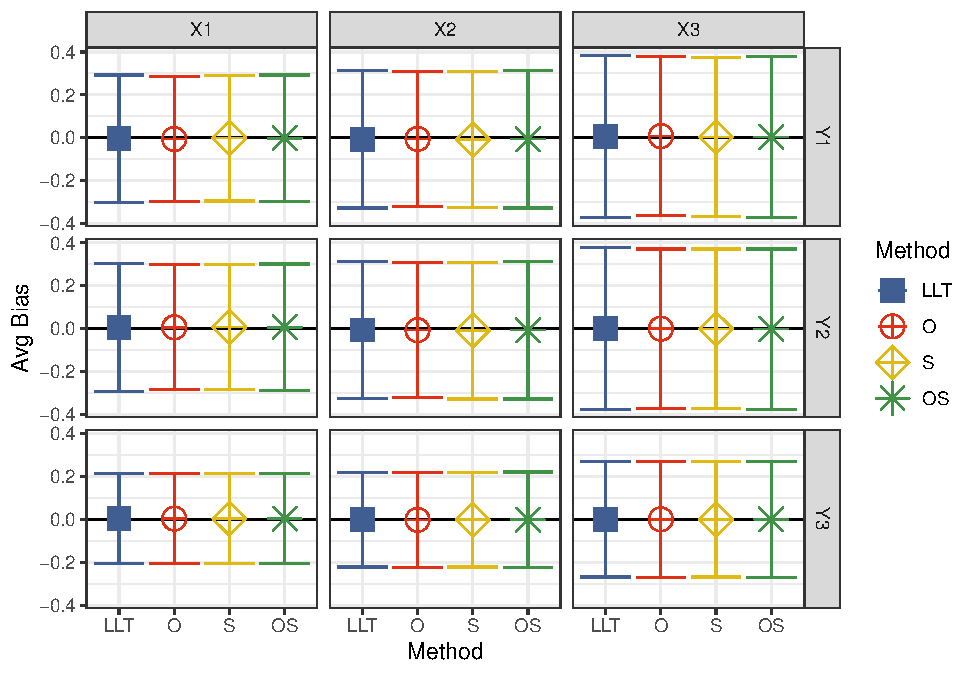
\includegraphics{FullSimulation_files/figure-latex/unnamed-chunk-15-1.pdf}
\caption{\label{fig:unnamed-chunk-15}Parameter Bias and Variablilty}
\end{figure}

\begin{longtable}[t]{l|r|l|r|l|r}
\caption{\label{tab:unnamed-chunk-16}Observation Covariance Estimates}\\
\hline
param & true & LLT & O & S & OS\\
\hline
1,1 & 15 & 14.866 & 15.248 & 15.147 & 15.065\\
\hline
1,2 & 0 & - & 2.436 & - & -0.387\\
\hline
2,2 & 15 & 14.908 & 15.293 & 15.18 & 15.092\\
\hline
1,3 & 0 & - & 0.012 & - & 0.006\\
\hline
2,3 & 0 & - & -0.020 & - & -0.033\\
\hline
3,3 & 10 & 10.06 & 10.064 & 10.087 & 10.102\\
\hline
\end{longtable}

\begin{longtable}[t]{l|l|r|l|r}
\caption{\label{tab:unnamed-chunk-17}Observation Covariance Coverage}\\
\hline
param & LLT & O & S & OS\\
\hline
1,1 & 0.949 & 0.949 & 0.938 & 0.935\\
\hline
1,2 & - & 0.029 & - & 0.904\\
\hline
2,2 & 0.95 & 0.935 & 0.936 & 0.935\\
\hline
1,3 & - & 0.959 & - & 0.955\\
\hline
2,3 & - & 0.952 & - & 0.946\\
\hline
3,3 & 0.945 & 0.948 & 0.948 & 0.947\\
\hline
\end{longtable}

\begin{longtable}[t]{l|r|l|l|r|r}
\caption{\label{tab:unnamed-chunk-18}State Covariance Estimates}\\
\hline
param & true & LLT & O & S & OS\\
\hline
1,1 & 5.000 & 4.879 & 4.59 & 4.803 & 4.940\\
\hline
1,2 & 3.714 & - & - & 3.786 & 3.980\\
\hline
2,2 & 5.000 & 4.899 & 4.606 & 4.838 & 4.977\\
\hline
1,3 & 0.000 & - & - & 0.017 & 0.015\\
\hline
2,3 & 0.000 & - & - & 0.003 & 0.015\\
\hline
3,3 & 2.000 & 1.89 & 1.932 & 1.916 & 1.928\\
\hline
\end{longtable}

\begin{longtable}[t]{l|l|l|r|r}
\caption{\label{tab:unnamed-chunk-19}State Covariance Coverage}\\
\hline
param & LLT & O & S & OS\\
\hline
1,1 & 0.932 & 0.908 & 0.922 & 0.930\\
\hline
1,2 & - & - & 0.946 & 0.918\\
\hline
2,2 & 0.937 & 0.902 & 0.913 & 0.911\\
\hline
1,3 & - & - & 0.951 & 0.935\\
\hline
2,3 & - & - & 0.950 & 0.933\\
\hline
3,3 & 0.927 & 0.937 & 0.922 & 0.927\\
\hline
\end{longtable}

\hypertarget{os-model-1}{%
\paragraph{OS Model}\label{os-model-1}}

\begin{longtable}[t]{l|l|r|r|r|r|r}
\caption{\label{tab:unnamed-chunk-20}Linear Effect Coverage}\\
\hline
Test & Variable & Beta & LLT & O & S & OS\\
\hline
Y1 & X1 & 4 & 0.962 & 0.948 & 0.968 & 0.961\\
\hline
Y1 & X2 & 2 & 0.946 & 0.934 & 0.955 & 0.945\\
\hline
Y1 & X3 & 1 & 0.952 & 0.941 & 0.958 & 0.950\\
\hline
Y2 & X1 & -3 & 0.950 & 0.944 & 0.958 & 0.957\\
\hline
Y2 & X2 & 0 & 0.945 & 0.931 & 0.959 & 0.952\\
\hline
Y2 & X3 & 1 & 0.949 & 0.940 & 0.968 & 0.964\\
\hline
Y3 & X1 & 0 & 0.957 & 0.962 & 0.960 & 0.957\\
\hline
Y3 & X2 & 0 & 0.950 & 0.947 & 0.949 & 0.952\\
\hline
Y3 & X3 & 0 & 0.945 & 0.948 & 0.949 & 0.949\\
\hline
\end{longtable}

\begin{figure}
\centering
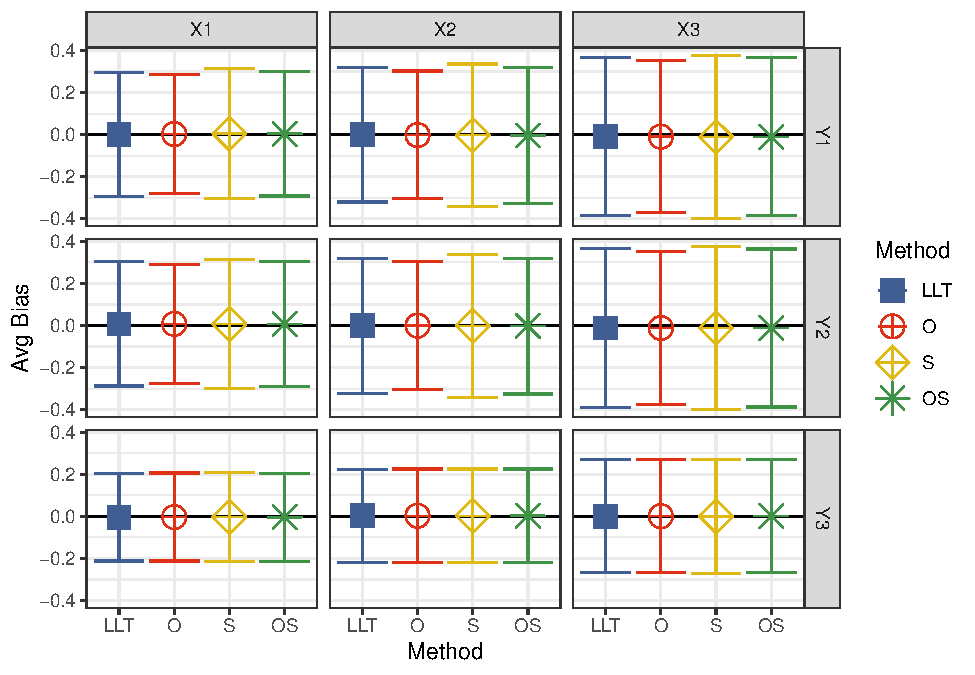
\includegraphics{FullSimulation_files/figure-latex/unnamed-chunk-21-1.pdf}
\caption{\label{fig:unnamed-chunk-21}Parameter Bias and Variablilty}
\end{figure}

\begin{longtable}[t]{l|r|l|r|l|r}
\caption{\label{tab:unnamed-chunk-22}Observation Covariance Estimates}\\
\hline
param & true & LLT & O & S & OS\\
\hline
1,1 & 15.0 & 14.964 & 15.752 & 14.273 & 15.075\\
\hline
1,2 & 2.4 & - & 4.976 & - & 2.140\\
\hline
2,2 & 15.0 & 14.948 & 15.733 & 14.248 & 15.066\\
\hline
1,3 & 1.0 & - & 0.997 & - & 0.979\\
\hline
2,3 & 1.0 & - & 1.008 & - & 0.997\\
\hline
3,3 & 10.0 & 10.021 & 10.021 & 9.988 & 10.056\\
\hline
\end{longtable}

\begin{longtable}[t]{l|l|r|l|r}
\caption{\label{tab:unnamed-chunk-23}Observation Covariance Coverage}\\
\hline
param & LLT & O & S & OS\\
\hline
1,1 & 0.944 & 0.882 & 0.867 & 0.943\\
\hline
1,2 & - & 0.024 & - & 0.917\\
\hline
2,2 & 0.941 & 0.879 & 0.851 & 0.938\\
\hline
1,3 & - & 0.946 & - & 0.942\\
\hline
2,3 & - & 0.948 & - & 0.926\\
\hline
3,3 & 0.937 & 0.935 & 0.937 & 0.931\\
\hline
\end{longtable}

\begin{longtable}[t]{l|r|l|l|r|r}
\caption{\label{tab:unnamed-chunk-24}State Covariance Estimates}\\
\hline
param & true & LLT & O & S & OS\\
\hline
1,1 & 5.000 & 4.835 & 4.168 & 5.776 & 4.941\\
\hline
1,2 & 3.714 & - & - & 5.007 & 3.891\\
\hline
2,2 & 5.000 & 4.849 & 4.183 & 5.800 & 4.952\\
\hline
1,3 & 0.000 & - & - & 0.470 & -0.009\\
\hline
2,3 & 0.000 & - & - & 0.470 & -0.015\\
\hline
3,3 & 2.000 & 1.894 & 1.943 & 1.977 & 1.939\\
\hline
\end{longtable}

\begin{longtable}[t]{l|l|l|r|r}
\caption{\label{tab:unnamed-chunk-25}State Covariance Coverage}\\
\hline
param & LLT & O & S & OS\\
\hline
1,1 & 0.94 & 0.78 & 0.828 & 0.942\\
\hline
1,2 & - & - & 0.447 & 0.937\\
\hline
2,2 & 0.924 & 0.789 & 0.820 & 0.927\\
\hline
1,3 & - & - & 0.719 & 0.938\\
\hline
2,3 & - & - & 0.738 & 0.939\\
\hline
3,3 & 0.926 & 0.938 & 0.930 & 0.930\\
\hline
\end{longtable}

\end{document}
